%% This is a skeleton file demonstrating the use of IEEEtran.cls (requires IEEEtran.cls version 1.8a or later) with an IEEE conference paper.
%%
%% Modified by Khan Reaz( kahn.reaz@ieee.org)
%% Support sites:
%% http://www.ieee.org/

%%***********************************************************
%% Legal Notice:
%% This code is offered as-is without any warranty either expressed or implied; without even the implied warranty of MERCHANTABILITY or FITNESS FOR A PARTICULAR PURPOSE! 
%% User assumes all risk and can modify as s/he wants.

%%***********************************************************

%package list
\documentclass[conference]{IEEEtran}
\usepackage{cite}
\usepackage{graphicx}
\graphicspath{ {images/} }
\usepackage[brazil]{babel}
\usepackage[utf8]{inputenc}

\begin{document}

\title{Análise de classificadores}
\author{Aryane Ast dos Santos}


%Authors List

\author
{\IEEEauthorblockN{Aryane Ast dos Santos}
\IEEEauthorblockA{Departamento de Informática\\
Universidade Federal do Paraná\\
Email: aras10@inf.ufpr.br}
}

\maketitle


%Main body starts

\begin{abstract}
Abstract goes here

\end{abstract}


\begin {IEEEkeywords}
IoT, Ontology, Semantics,  SSN, OWL, OBOE, OpenIoT, SWEET, SUMO
\end{IEEEkeywords}


\section{Introdução}

Um problema de classificação consiste em definir um rótulo ou classe para um
elemento a partir de um conjunto de elemento com rótulos definidos. Motivação
por favor.

Este relatório se propõe a apresentar resultados obtidos com os classificadores
KNN (K Nearest Neighbors), Naive Bayes, Árvores de Decisão e Support Vector
Machines num problema de classificação de imagens. A base utilizada contém 1901
imagens rotuladas em 9 classes diferentes. Os algoritmos de classificação não
utilizam as imagens brutas, de forma que é necessário converter as imagens do
formato JPG para vetores de características que os algoritmos de classificação
possam utilizar.



%,
%formando então uma base de treinamento, que denominei "completa", contendo o
%vetor de características que representa a imagem e seu rótulo respectivo.

Após ter o vetor de características, são realizados as execuções dos
classificadores KNN, Naive Bayes e de Árvores de Decisão para todas as bases
de treinamento e validação, e então o desempenho de cada classificador é
apresentado.

Nas seções a seguir são apresentados maiores detalhes em como obter
representações dos dados, os métodos utilizados, as métricas para desempenho,
etc, etc.

\section{Representação dos dados}

Para cada uma das imagens disponibilizadas para classificação, é realizada uma
extração de características, no caso histograma de cores e contorno da imagem,
why?
Para a extração dos vetores de caracteristicas, foi utilizada o script
create\_bases.py, que pode ser visualizado no código abaixo (ref das linhas x a
y).

\subsection{Outro.. LBP?}
Explicação

%código create_bases.py

Após extração dos vetores de características, é realizada uma separação
aleatória de todos os vetores de características em bases de
treinamento e de validação, cada uma com 60\% e 40\% da completa,
respectivamente. Essa separação é realizada com o script em Bash com o script
generate\_train\_test.sh, que, essencialmente faz 


\section{


show code, baby

\section{Considerações Finais}

Todo o código utilizado no projeto, inclusos ..., pode ser encontrado num
repositório Git hospedado no GitHub ....

%\section{Introduction}
%\label{intro}
%Here goes the introduction
%
%%example for Bullet point list
%
%\begin{itemize}
%\item example
%\end {itemize}
%
%%example for numbered list
%    \begin{enumerate}
%    \item example
%    \end{enumerate}
%
%%example for inserting image
%\begin{figure}[h]
%   \centering
%   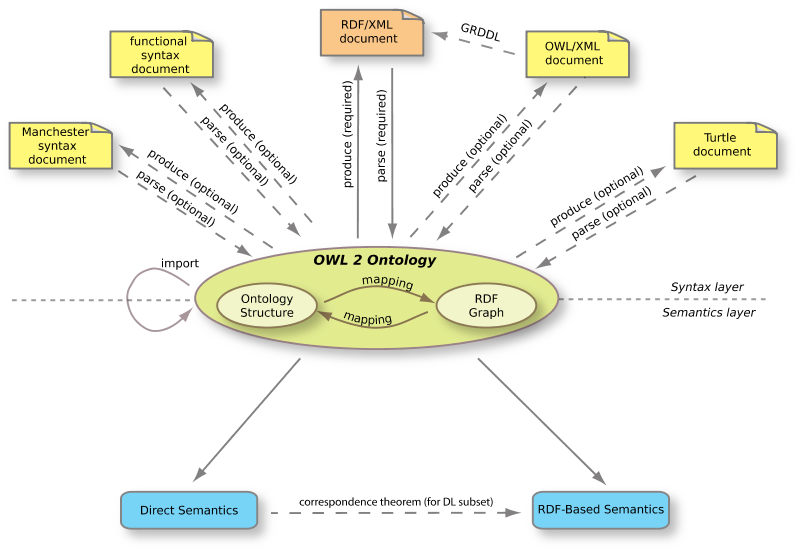
\includegraphics[scale=.45]{OWL2}
%    \caption{The structure of OWL2}
%    \label{fig:OWL2}
%\end{figure}
%
%\section{Conclusion}
%\label {conclusion}
%\input{sections/5_conclusion.tex}
%
%\bibliographystyle{IEEEtran}
%\bibliography{bibliography}

\end{document}
